\chapter{Método espectral e Método dos elementos finitos}
\label{cap:I}
\section{Método espectral} 

 Método espectral é um método poderoso usado para solução de equações diferencial parcial. Diferentemente do método das diferenças finitas, que considera apenas os pontos próximos do ponto que queremos computar chamada de método \emph{local}, o método espectral considera todo o domínio, sendo assim um método \emph{global}. Essa técnica tem mais precisão pois converge exponencialmente diferente do método local. É preferível a utilização desse método quando a solução varia em função do \textit{tempo} e \textit{espaço}. \corr{E o método de elementos espectrais?}

\section{Interpolação}
 A interpolação de uma função $f(x)$ por um polinômio trigonométrico ou não, de grau $n$, $P_{n}(x)$ e que satisfaça:

\begin{equation}
	P_n (x_i) = f(x_i) \ i = 1,2,...,\emph{n+1}
\end{equation}

 Onde $f(x_i)$ é a função $f$ pré-calculada nos pontos $x_i$. A escolha desses pontos $x_i$ ainda será explicada.

\subsection{Interpolação polinomial}
 \begin{figure}[!ht]
  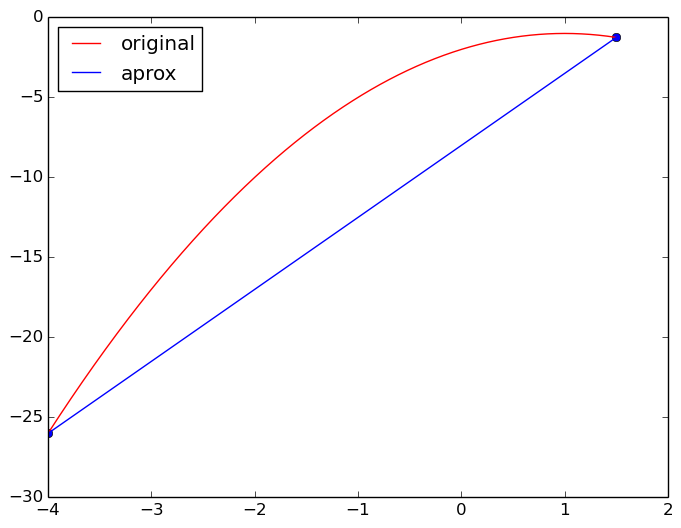
\includegraphics[width=0.7\textwidth,center]{figuras/interpolacao_linear.png}
  \caption{interpolação simples}
\end{figure}

 Antes do uso de calculadoras e computadores, um método de estimar o valor de uma $f$ num ponto, era utilizar tabelas com valores de pré-calculados. \corr{A maneira mais simples de entender é a estimação do valor da função em um ponto intermediário entre dois pontos conhecidos é o uso da interpolação \emph{Linear}}.

\begin{equation}
	f(x) \approx \frac{x - x_1}{x_0 - x_1}f(x_0)  + \frac{x - x_0}{x_1 - x_0}f(x_1)
\end{equation} 
 
 Para fazermos essa interpolação para $n$ pontos conhecidos aproximamos uma função usando o polinômio base de \emph{Lagrange}.
\begin{equation}
C_i(x) = \prod_{j = 0 \\ j \neq i}^{N} \frac{x - x_j}{x_i - x_j} 
\end{equation}

\begin{figure}[!h]
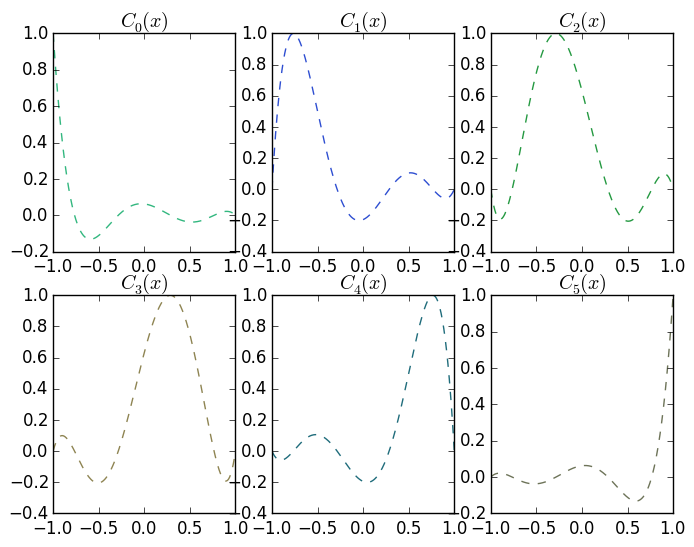
\includegraphics[width=0.7\textwidth, center ]{figuras/exemplo_polinomio_lagrange.png}
\caption{polinômio base de Lagrange para 6 pontos}
\end{figure}

 A interpolação de \emph{Lagrange} é dada por :
\begin{equation}
 P_n(x) \equiv \sum_{i = 0}^{N} f(x_i)C_i(x) 
\end{equation}
 Obedecendo que $P_n(x_i) = f(x_i)$. Apesar dos pontos interpoladores equidistante serem comumente utilizados, não há restrições, podendo até mesmo estar fora de ordem.
\begin{figure}[h]
  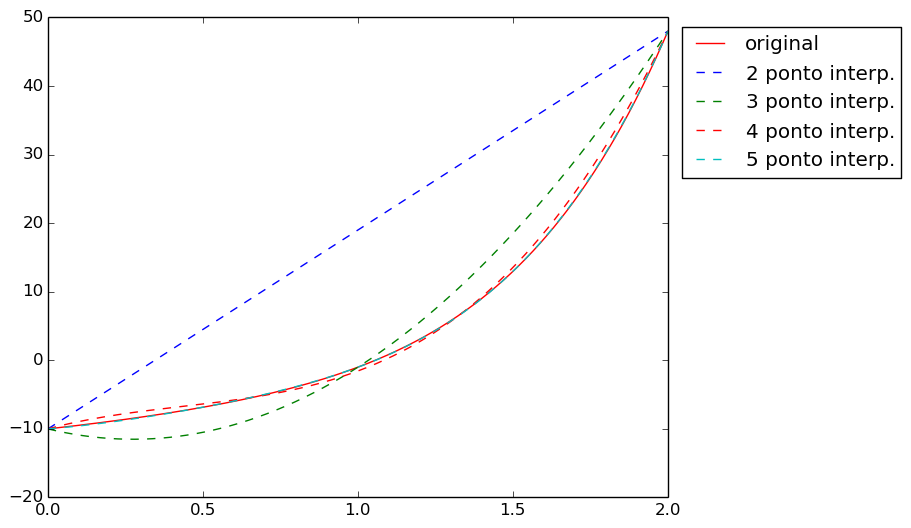
\includegraphics[width=0.5\textwidth, center]{figuras/interpolacao_linear5.png}
  \caption{interpolação com n pontos equidistantes}
\end{figure}

\pagebreak
\newpage

\subsection{Fenômeno de Runge}
 Apesar de parecer que uma boa interpolação tenha uma boa aproximação usando pontos igualmente distantes sobre um interval $[a,b]$, $\lim_{n \rightarrow \infty} |f(x) - P_n(x)| = 0$ para qualquer $f(x)$ diferenciável.
 No início do século XX, \emph{Carl David Tolmé Runge}, provou que para uma função $f(x)$:
 \begin{equation}
 f(x) = \frac{1}{1 + x^2} , x \in [-5,5]
 \end{equation}
 que para pontos equidistantes, a interpolação converge apenas no intervalo $[-3.63,3.63]$, e diverge fora do mesmo. Para polinômios de maior grau, esse intervalo de convergência tende a diminuir e perto dos pontos de fronteira diverge bastante (figura abaixo).

\begin{figure}[htp]
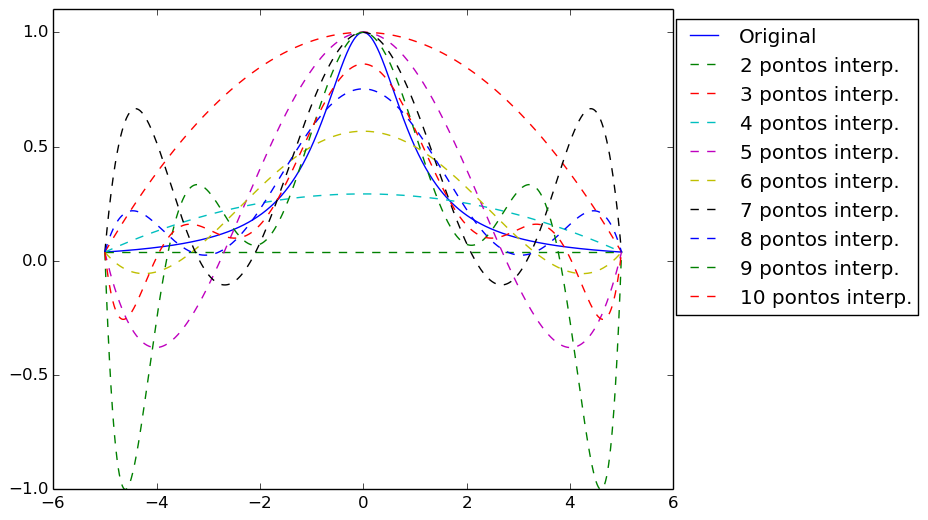
\includegraphics[width=0.7\textwidth, center]{figuras/fenomeno_runge.png}
\caption{fenômeno Runge}
\end{figure}

 Assim, Runge prova que no meio do intervalo temos boas aproximações mas infelizmente perto dos extremos, os valores interpolados oscilam muito, para um polinômio de grau n com pontos equidistante. Esse fenômeno sugere que escolhamos pontos diversos que tenham menor concentração do meio do intervalo, onde temos uma maior precisão, e aumentar a densidade de pontos próximos dos extremos.
 Agora como encontrar uma distribuição de pontos de forma que melhore a interpolação ? A resposta pode ser explicado pelos teoremas a seguir.
\pagebreak
\subsection{ Teorema I: Erro de interpolação de Cauchy}

 Dado $f(x)$  com pelo menos $N+1$ derivadas no intervalo de interesse e seja $P_N(x)$ seja o interpolador Lagrangiano de grau $N$. Então o erro é dado por:
 
 \begin{equation}
 f(x) - P_N(x) = \frac{1}{[N+1]!}f^{(N+1)}(\epsilon)\prod^{N}_{i = 0} (x - x_i)
 \end{equation}
 Para um $\epsilon(x) \in [-1,1]$.
 
 Logo, para minimizar o erro, não podemos fazer nada quanto o termo $f^{(N+1)}(\epsilon)$, pois necessita conhecer a função interpolada. Quanto o polinômio $\prod^{N}_{i = 0} (x - x_i)$, sabemos que o coeficiente do termo $x^N$ é $1$, independente da escolha de pontos. Então a pergunta que fica é, qual escolha de pontos nos dá um \emph{polinômio} com coeficiente líder igual a $1$ minimiza essa função ? Felizmente e coincidentemente, essa resposta foi respondida quase meio século antes do próprio fenômeno de Runge ser descoberto. Veremos no próximo teorema.

 
\subsection{Teorema II: Amplitude minima}
 De todos os polinômios de grau $N$ com coeficiente de $x^N$ igual a 1, o único polinômio que tem o menor máximo no intervalo $[-1,1]$ é $\frac{T_N(x)}{2^{N-1}}$, o polinômio de \emph{Chebyshev}  dividido por $2^{N-1}$. Em outras palavras, todos os polinômios de mesmo grau e coeficiente líder unitário,chamados de polinômios mônicos, satisfazem a desigualdade:

\begin{equation}
	max_{x \in [-1,1]}|P_N(x)| \geq  max_{x \in [-1,1]} \left |\frac{T_N(x)}{2^{N-1}}  \right |  = \frac{1}{2^{N-1}}\\
\end{equation}

\begin{align}
    &T_0(x) = 1\\
    &T_1(x) = x\\
    &T_{N+1}(x) = 2xT_N(x) - T_{N-1}(x)\\
    &T_{N}(x) =\cos(n \arccos x)=\cosh(n\,\operatorname{arcosh}\,x)
\end{align}

 Agora, qualquer polinômio de grau $N$, com coeficiente líder unitário, pode ser fatorado na forma de um produtório  $(x - x_i)$, onde $x_i$ é uma das raízes do polinômio, em particular: 
 \begin{equation}
 \frac{1}{2^N}T_{N+1}(x) \equiv \prod_{i = 1}^{N+1} (x-x_i)
 \end{equation}
 Temos então que, para minimizar o erro no \emph{Teorema I}, o polinômio deve ser proporcional a $T_{N+1}(x)$. Isso implica que  os pontos interpoladores que minimizam o erro, são as raízes do próprio polinômio de \emph{Chebyshev} de grau $N+1$.
 
 Usando o fato que esse polinômio pode ser reescrita como uma função trigonométrica, temos que as raízes são:
 \begin{equation}
  x_i  \equiv \cos \left [ \frac{(2i - 1)\pi}{2(N+1)}  \right ] , i = 1,2,..., N+1
 \end{equation}
 
 Pela expansão de \emph{Taylor} da função coseno, verificamos a afirmação de acima que o espaçamento da malha é $O(N^2)$ perto das fronteiras:
 
 \begin{equation}
  x_1 \approx -1 + \frac{\pi^2}{8N^2}\ ;\ x_2 \approx -1 + \frac{9\pi}{8N^2}\ \ [N\gg 1]
 \end{equation}
 
 Agora temos como conseguir o polinômio de \emph{Chebyshev} que minimiza o erro. Porém essa escolha de polinômio varia para diferentes geometrias ou funções harmônicas ou hermitianas.
 \begin{figure}[t]
 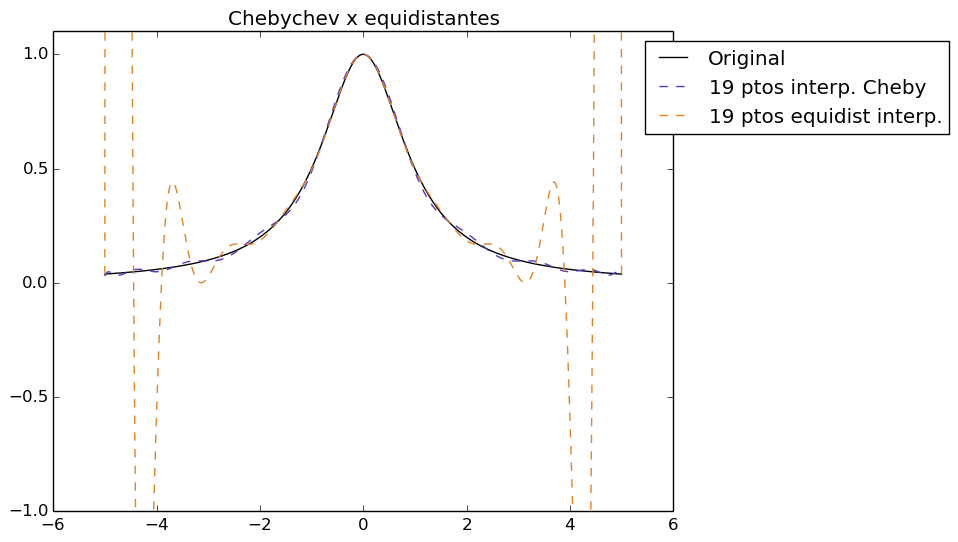
\includegraphics[width=0.45\textwidth, center]{figuras/chebychev_equidist.png}
 \caption{método de raízes de Chebychev contra raízes de pontos equidistante}
 \end{figure}
\pagebreak
\section{Integração numérica}
 Usando um polinômio interpolador $P$ de grau menor ou igual a $n$ na forma de Lagrange, podemos escrever a integral de $f$ no intervalo $[a,b]$:\\
 
\begin{equation}
\int^{a}_b f(x) \partial x\ = \int^{a}_b[\sum_{i\ =\ 0}^N P_i(x) f(x_i)]\ \partial x +  \int^{a}_b \prod_{i\ =\ 0} (x - x_i)\frac{f^{(n+1)}(\varepsilon)}{(n+1)!}\ \partial x\\
\end{equation}

podemos aproximar a integral por:
\begin{equation}
   \int^{a}_b f(x) \partial x\ \approx \sum_{i\ =\ 0}^N f(x_i) \int^{a}_b P_i(x) \partial x\ =\ \sum_{i\ =\ 0}^N f(x_i) w_i \\
\end{equation}

onde o coeficiente é:
\begin{equation}
 w_i =  \int^{a}_b  P_i(x) 
\end{equation}
 E esse coeficiente independem da função $f$ e são somente depende dos pontos $x_i$ considerados. Estes pontos $x_i$ são determinados de modo a tornar o erro nulo quando integrarmos uma função que é um polinômio quando integrarmos uma função que é um polinômio de grau menor ou igual a $(2n +1)$.
 Tomemos $f$ como sendo um polinômio de grau $(2n+1)$.Desta forma a derivada de ordem (n+1) da função $f$ será um polinômio de grau n. Logo, utilizamos o polinômio, $P$ para interpolá-lo:
 \begin{equation}
 f^{n+1}(x) = \sum^{n}_{j = 0} b_j P_j(x)
 \end{equation}
 E também para interpolar o termo $\prod^{n}_{i = 0} (x - x_j)$:
\begin{equation}
 \prod^{n}_{i = 0} (x - x_j) =  P_{n+1}(x)
\end{equation}  
Assim, fazemos:
\begin{equation}
\int^{a}_b \prod_{i\ =\ 0} (x - x_i)\frac{f^{(n+1)}(\varepsilon)}{(n+1)!}\ \partial x = \sum^{n}_{j = 0} b_j \int^{a}_b   P_{n+1}(x) P_j(x) \partial x
\end{equation}
 Agora, seja o polinômio $P$ ortogonal  em relação ao produto escalar:
\begin{equation}
 (f,g) = \int^b_a f(x)g(x) \partial x
\end{equation}
 Assim anulamos o erro:
\begin{align}
&(P_i,P_j) = \int^b_a P_i(x) P_j(x) \partial x = 0\ ,\ i \neq j\\
&\int^{a}_b \prod_{i\ =\ 0} (x - x_i)\frac{f^{(n+1)}(\varepsilon)}{(n+1)!}\ \partial x = \sum^{n}_{j = 0} b_j \int^{a}_b   P_{n+1}(x) P_j(x) \partial x = 0
\end{align}

 No caso acima foi utilizado para a integração um polinômio qualquer ortogonal, porém podemos utilizar qualquer classe de polinômios \emph{ortogonais} para estimarmos a integral da função, tomando os zeros dos polinômios a nossa escolha.[\emph{Gauss-Chebychev}, \emph{Gauss-Jacobi}, \emph{Gauss-Radau}, \emph{Gauss-Lobatto}]
\section{Derivada}


\section{Método Pseudo-espectralou da colocação}

\section{Método de Galerkin}

\section{método dos elementos finitos}
adicionar texto de elementos dinâmicos